\section{Mức độ 5,6 điểm}
\begin{dang}{Tính diện tích xung quanh, diện tích toàn phần, chiều cao, bán kính đáy. Thiết diện.}
\end{dang}
\Opensolutionfile{ans}[ans/CD22/Muc_5_6]
\begin{ex}%[2H2Y1-2]%[Đề tham khảo 2020 Lần 2] 
	Diện tích xung quanh của hình trụ có độ dài đường sinh $\ell$ và bán kính đáy $r$ bằng
	\choice
	{$4\pi r\ell$}
	{$\pi r\ell$}
	{$\dfrac{1}{3}\pi r\ell$}
	{\True $2\pi r\ell$}
	\loigiai
	{Diện tích xung quanh của hình trụ $S=2\pi r\ell$.}
\end{ex}
\begin{ex}%[2H2Y1-2]%[Mã 101 - 2020 lần 1] 
	Cho hình trụ có bán kính đáy $r=8$ và độ dài đường sinh $\ell=3$. Diện tích xung quanh của hình trụ đã cho bằng
	\choice
	{$24\pi$}
	{$192\pi$}
	{\True $48\pi$}
	{$64\pi$}
	\loigiai
	{Diện tích xung quanh của hình trụ $S=2\pi r\ell=48\pi$.}
\end{ex}
\begin{ex}%[2H2Y1-2]%[Mã 102 - 2020 lần 1]
	Cho hình trụ có bán kính đáy $r=4$ và độ dài đường sinh $\ell=3$. Diện tích xung quanh của hình trụ đã cho bằng
	\choice
	{$48\pi$}
	{$12\pi$}
	{$16\pi$}
	{\True $24\pi$}
	\loigiai
	{Diện tích xung quanh của hình trụ $S=2\pi r\ell=2\pi.4.3=24\pi$.}
\end{ex}
\begin{ex}%[2H2Y1-2]%[Mã 103 - 2020 lần 1] 
	Cho hình trụ có bán kính đáy $r=5$ và độ dài đường sinh $\ell=3$. Diện tích xung quanh của hình trụ đã cho bằng
	\choice
	{$15\pi$}
	{$25\pi$}
	{\True $30\pi$}
	{$75\pi$}
	\loigiai
	{Diện tích xung quanh của hình trụ $S=2\pi r\ell=30\pi$.}
\end{ex}
\begin{ex} %[2H2Y1-2]%[Mã 104 - 2020 lần 1]
	Cho hình trụ có bán kính đáy $r=7$ và độ dài đường sinh $\ell=3$. Diện tích xung quanh của hình trụ đã cho bằng
	\choice
	{\True $42\pi$}
	{$147\pi$}
	{$49\pi$}
	{$21\pi$}
	\loigiai
	{Diện tích xung quanh của hình trụ $S=2\pi r\ell=42\pi$.}
\end{ex}
\begin{ex} %[2H2K1-2]%[Đề minh họa 2020 lần 1]
	Cho hình trụ có bán kính đáy bằng 3. Biết rằng khi cắt hình trụ đã cho bởi một mặt phẳng qua trục, thiết diện thu được là một hình vuông. Diện tích xung quanh của hình trụ đã cho bằng
	\choice
	{$18\pi$}
	{\True $36\pi$}
	{$54\pi$}
	{$27\pi$}
	\loigiai
	{\begin{center}
			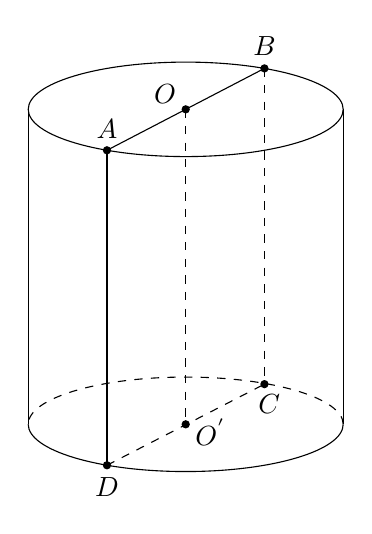
\begin{tikzpicture}
				\draw (0,0) ellipse (2cm and 0.6cm);
				\draw (-2,0) -- (-2,-4);
				\draw (2,0) -- (2,-4);
				\draw (-2,-4) arc (180:360:2cm and 0.6cm);
				\draw[dashed] (2,-4) arc (0:180:2cm and 0.6cm);
				\node[left] at (0,0.2) {\normalsize$O$};
				\fill (0,0) circle (1.5pt);
				\node[right] at (0,-4.1) {\normalsize$O^{'}$};
				\fill (0,-4) circle (1.5pt);
				\draw[dashed] (0,0) -- (0,-4);
				\fill (1,0.52) circle (1.5pt);
				\node at (-1,-0.25) {\normalsize$A$};
				\fill (-1,-0.52) circle (1.5pt);
				\node at (1,0.8) {\normalsize$B$};
				\draw (1,0.52) -- (-1,-0.52);
				\fill (1,-3.49) circle (1.5pt);
				\node[below right] at (0.8,-3.5) {\normalsize$C$};
				\fill (-1,-4.52) circle (1.5pt);
				\node at (-1,-4.8) {\normalsize$D$};
				\draw[dashed] (-1,-4.52) -- (1,-3.49);
				\draw[dashed] (1,0.52) -- (1,-3.49);
				\draw (-1,-0.52) -- (-1,-4.52);
			\end{tikzpicture}
		\end{center}
		Giả sử thiết diện qua trục của hình trụ là hình vuông $ABCD$.\\
		Theo giả thiết ta có bán kính đáy của hình trụ là $r=3\Rightarrow h=AD=DC=2r=6=\ell$.\\
		Vậy diện tích xung quanh của hình trụ là: $S_{\text{sq}}=2\pi r\ell=2\pi .3.6=36\pi$.}
\end{ex}
\begin{ex}%[2H2K1-2]%[Đề minh họa 2017]
	Trong không gian, cho hình chữ nhật $ABCD$ có $AB=1$ và $AD=2$. Gọi $M,N$ lần lượt là trung điểm của $AD$ và $BC$. Quay hình chữ nhật $ABCD$ xung quanh trục $MN$, ta được một hình trụ. Diện tích toàn phần $S_{tp}$ của hình trụ đã cho bằng
	\choice
	{$S_{\text{tp}}=10\pi$}
	{$S_{\text{tp}}=2\pi$}
	{$S_{\text{tp}}=6\pi$}
	{\True $S_{\text{tp}}=4\pi$}
	\loigiai
	{\begin{center}
			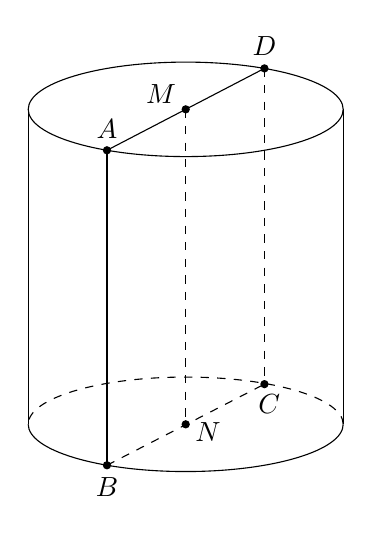
\begin{tikzpicture}
				\draw (0,0) ellipse (2cm and 0.6cm);
				\draw (-2,0) -- (-2,-4);
				\draw (2,0) -- (2,-4);
				\draw (-2,-4) arc (180:360:2cm and 0.6cm);
				\draw[dashed] (2,-4) arc (0:180:2cm and 0.6cm);
				\node[left] at (0,0.2) {\normalsize$M$};
				\fill (0,0) circle (1.5pt);
				\node[right] at (0,-4.1) {\normalsize$N$};
				\fill (0,-4) circle (1.5pt);
				\draw[dashed] (0,0) -- (0,-4);
				\fill (1,0.52) circle (1.5pt);
				\node at (-1,-0.25) {\normalsize$A$};
				\fill (-1,-0.52) circle (1.5pt);
				\node at (1,0.8) {\normalsize$D$};
				\draw (1,0.52) -- (-1,-0.52);
				\fill (1,-3.49) circle (1.5pt);
				\node[below right] at (0.8,-3.5) {\normalsize$C$};
				\fill (-1,-4.52) circle (1.5pt);
				\node at (-1,-4.8) {\normalsize$B$};
				\draw[dashed] (-1,-4.52) -- (1,-3.49);
				\draw[dashed] (1,0.52) -- (1,-3.49);
				\draw (-1,-0.52) -- (-1,-4.52);
			\end{tikzpicture}
		\end{center}
		Quay hình chữ nhật $ABCD$ xung quanh $MN$ nên hình trụ có bán kính $r=AM=\dfrac{AD}{2}=1$.\\
		Vậy diện tích toàn phần của hình trụ $S_{\text{tp}}=2\pi r.AB+2\pi r^2=2\pi +2\pi=4\pi$.}
\end{ex}
\begin{ex}%[2H2B1-2]%[Mã 105 2017]
	Cho hình trụ có diện tích xung quanh bằng $50\pi$ và độ dài đường sinh bằng đường kính của đường tròn đáy. Bán kính $r$ của đường tròn đáy đã cho bằng
	\choice
	{$r=5\sqrt{\pi}$}
	{$r=5$}
	{$r=\dfrac{5\sqrt{2\pi}}{2}$}
	{\True $r=\dfrac{5\sqrt{2}}{2}$}
	\loigiai
	{Diện tích xung quanh của hình trụ là $S_{\text{xq}}=2\pi r\ell\leftrightarrow2\pi r\ell=50\pi\leftrightarrow2\pi r.2r=50\pi\leftrightarrow r=\dfrac{5\sqrt{2}}{2}$.}
\end{ex}
\begin{ex}%[2H2B1-2]%[Chuyên lam Sơn Thanh Hóa 2019]
	Cho khối trụ $(T)$ có bán kính đáy $r=1$, thể tích $V=5\pi$. Diện tích toàn phần của hình trụ tương ứng bằng
	\choice
	{\True $S_{\text{tp}}=12\pi$}
	{$S_{\text{tp}}=11\pi$}
	{$S_{\text{tp}}=10\pi$}
	{$S_{\text{tp}}=7\pi$}
	\loigiai
	{Ta có $V=S_{\text{đáy}}.h$ với $S_{\text{đáy}}=\pi r^2=\pi$ nên $h=\dfrac{V}{S_{\text{đáy}}}=5$.\\
		Diện tích toàn phần của hình trụ tương ứng là $S_{\text{tp}}=2\pi rh+2\pi r^2=2\pi 1.5+2\pi 1^2=12\pi$.}
\end{ex}
\begin{ex}%[2H2Y1-2]%[THPT lê Quý Đôn Điện Biên 2019]
	Diện tích xung quanh của hình trụ biết hình trụ có bán kính đáy là $a$ và đường cao là $a\sqrt{3}$ bằng
	\choice
	{$2\pi a^2$}
	{$\pi a^2$}
	{$\pi a^2\sqrt{3}$}
	{\True $2\pi a^2\sqrt{3}$}
	\loigiai
	{Diện tích xung quanh của hình trụ là $S_{\text{xq}}=2\pi rh=2\pi .a.a\sqrt{3}=2\pi a^2\sqrt{3}$.}
\end{ex}
%%--11-20
\begin{ex}%[2H2B1-2]
	Cắt một khối trụ bởi một mặt phẳng qua trục của nó ta được thiết diện là một hình vuông có cạnh bằng $3a$. Tính diện tích toàn phần của khối trụ.
	\choice
	{$S_{tp}= \dfrac{13\pi a^2}{6}$}
	{$S_{tp}= \sqrt3\pi a^2$}
	{$S_{tp}= \dfrac{\sqrt3\pi a^2}{2}$}
	{\True $S_{tp}= \dfrac{27\pi a^2}{2}$}
	\loigiai{
		\immini{
			Thiết diện qua trục là một hình vuông có cạnh bằng $3a$ nên ta có độ dài đường sinh $\ell =3a$ và bán kính đường tròn đáy là $\dfrac{3a}{2}$.\\
			Từ đó ta tính được $S_{tp}= 2\pi r \ell + 2\pi r^2= \dfrac{27\pi a^2}{2}$.
		}{
			\begin{tikzpicture}[scale=1, font=\footnotesize, line join=round, line cap=round, >=stealth]
				\def\x{2} % Bán kính trụ lớn
				\pgfmathsetmacro{\y}{\x/4} % Bán kính trục bé
				\def\h{3} % Chiều cao
				\coordinate[label=right:$A$] (A) at (\x,0);
				\coordinate[label=below :$O$] (O) at (0,0);
				\coordinate[label=right:$A'$] (A') at ($(A)+(90:\h)$);
				\coordinate[label=above :$O'$] (O') at ($(O)+(90:\h)$);
				\coordinate[label=left:$B$] (B) at ($(A)!2!(O)$);
				\coordinate[label=left:$B'$] (B') at ($(A')!2!(O')$);
				\draw (B')--(O') (A) arc (0:-180:{\x} and {\y})--($(A')!2!(O')$) arc (180:0:{\x} and {\y}) arc (0:-180:{\x} and {\y}) (A)--(A')--(O');
				\draw[dashed] (B)--(O) (O')--(O)--(A) arc (0:180:{\x} and {\y});
				\foreach \diem in {A,A',O,O',B,B'}   \fill (\diem)circle(1.5pt);
			\end{tikzpicture}
		}
	}
\end{ex}

\begin{ex}%[2H2B1-2]
	Một hình trụ có diện tích xung quanh bằng $4\pi a^2$ và bán kính đáy là $a$. Tính độ dài đường cao của hình trụ đó. 
	\choice
	{$a$}
	{\True $2a$}
	{$3a$}
	{$4a$}
	\loigiai{
		\immini{
			Diện tích xung quanh của hình trụ có bán kính đáy $a$ và chiều cao $h$ là 
			$$S_{xq}= 2\pi a h \Leftrightarrow h= \dfrac{S_{xq}}{2\pi a}=2a.$$
			Vậy độ dài đường cao của hình trụ đó là $h= 2a$.
		}{
			\begin{tikzpicture}[scale=1, font=\footnotesize, line join=round, line cap=round, >=stealth]
				\def\x{2} % Bán kính trụ lớn
				\pgfmathsetmacro{\y}{\x/4} % Bán kính trục bé
				\def\h{3} % Chiều cao
				\coordinate[label=right:$A$] (A) at (\x,0);
				\coordinate[label=below :$O$] (O) at (0,0);
				\coordinate[label=right:$A'$] (A') at ($(A)+(90:\h)$);
				\coordinate[label=above :$O'$] (O') at ($(O)+(90:\h)$);
				\coordinate[label=left:$B$] (B) at ($(A)!2!(O)$);
				\coordinate[label=left:$B'$] (B') at ($(A')!2!(O')$);
				\draw (B')--(O') (A) arc (0:-180:{\x} and {\y})--($(A')!2!(O')$) arc (180:0:{\x} and {\y}) arc (0:-180:{\x} and {\y}) (A)--(A')--(O');
				\draw[dashed] (B)--(O) (O')--(O)--(A) arc (0:180:{\x} and {\y});
				\foreach \diem in {A,A',O,O',B,B'}   \fill (\diem)circle(1.5pt);
			\end{tikzpicture}
		}
	}
\end{ex}

\begin{ex}%[2H2B1-2]
	Một hình trụ có bán kính đáy bằng $2$ cm và có thiết diện qua trục là một hình vuông. Diện tích xung quanh của hình trụ là
	\choice
	{$8\pi\, \text{cm}^2$}
	{$4\pi\, \text{cm}^2$}
	{$32\pi\, \text{cm}^2$}
	{\True $16\pi\, \text{cm}^2$}
	\loigiai{
		\immini{
			Vì thiết diện qua trục là hình vuông nên ta có $h=2r=4$ cm.\\
			Công thức tính diện tích xung quanh hình trụ có bán kính đáy $r$, chiều cao $h$ là 
			$$S_{xq}= 2\pi rh= 16\pi\, \text{cm}^2$$
		}{
			\begin{tikzpicture}[scale=1, font=\footnotesize, line join=round, line cap=round, >=stealth]
				\def\x{2} % Bán kính trụ lớn
				\pgfmathsetmacro{\y}{\x/4} % Bán kính trục bé
				\def\h{3} % Chiều cao
				\coordinate[label=right:$A$] (A) at (\x,0);
				\coordinate[label=below :$O$] (O) at (0,0);
				\coordinate[label=right:$A'$] (A') at ($(A)+(90:\h)$);
				\coordinate[label=above :$O'$] (O') at ($(O)+(90:\h)$);
				\coordinate[label=left:$B$] (B) at ($(A)!2!(O)$);
				\coordinate[label=left:$B'$] (B') at ($(A')!2!(O')$);
				\draw (B')--(O') (A) arc (0:-180:{\x} and {\y})--($(A')!2!(O')$) arc (180:0:{\x} and {\y}) arc (0:-180:{\x} and {\y}) (A)--(A')--(O');
				\draw[dashed] (B)--(O) (O')--(O)--(A) arc (0:180:{\x} and {\y});
				\foreach \diem in {A,A',O,O',B,B'}   \fill (\diem)circle(1.5pt);
			\end{tikzpicture}
		}
	}
\end{ex}

\begin{ex}%[2H2B1-2]
	Cắt một hình trụ bởi một mặt phẳng qua trục của nó, ta được thiết diện là một hình vuông có cạnh bằng $3a$. Tính diện tích toàn phần của hình trụ đã cho. 
	\choice
	{$S_{tp}= \dfrac{13\pi a^2}{2}$}
	{\True $S_{tp}= \dfrac{27\pi a^2}{2}$}
	{$S_{tp}= 9\pi a^2$}
	{$S_{tp}= \dfrac{9\pi a^2}{2}$}
	\loigiai{
		\immini{
			Thiết diện qua trục là một hình vuông có cạnh bằng $3a$ nên ta có độ dài đường sinh $\ell =3a$ và bán kính đường tròn đáy là $\dfrac{3a}{2}$.\\
			Từ đó ta tính được $S_{tp}= 2\pi r \ell + 2\pi r^2= \dfrac{27\pi a^2}{2}$.
		}{
			\begin{tikzpicture}[scale=1, font=\footnotesize, line join=round, line cap=round, >=stealth]
				\def\x{2} % Bán kính trụ lớn
				\pgfmathsetmacro{\y}{\x/4} % Bán kính trục bé
				\def\h{3} % Chiều cao
				\coordinate[label=right:$A$] (A) at (\x,0);
				\coordinate[label=below :$O$] (O) at (0,0);
				\coordinate[label=right:$A'$] (A') at ($(A)+(90:\h)$);
				\coordinate[label=above :$O'$] (O') at ($(O)+(90:\h)$);
				\coordinate[label=left:$B$] (B) at ($(A)!2!(O)$);
				\coordinate[label=left:$B'$] (B') at ($(A')!2!(O')$);
				\draw (B')--(O') (A) arc (0:-180:{\x} and {\y})--($(A')!2!(O')$) arc (180:0:{\x} and {\y}) arc (0:-180:{\x} and {\y}) (A)--(A')--(O');
				\draw[dashed] (B)--(O) (O')--(O)--(A) arc (0:180:{\x} and {\y});
				\foreach \diem in {A,A',O,O',B,B'}   \fill (\diem)circle(1.5pt);
			\end{tikzpicture}
		}
	}
\end{ex}

\begin{ex}%[2H2B1-2]
	\immini{
		Trong không gian cho hình chữ nhật $ABCD$ có $AB=1,\, AD=2$. Gọi $M,\, N$ lần lượt là trung điểm của $AD$ và $BC$. Quay hình chữ nhật đó xung quanh trục $MN$ ta được một hình trụ. Tính diện tích toàn phần $S_{tp}$ của hình trụ đó.
		\choice
		{\True $S_{tp}=4\pi$}
		{$S_{tp}=6\pi$}
		{$S_{tp}=2\pi$}
		{$S_{tp}=10\pi$}
	}{
		\begin{tikzpicture}[scale=1, font=\footnotesize, line join=round, line cap=round, >=stealth]
			\def\x{2} % Bán kính trụ lớn
			\pgfmathsetmacro{\y}{\x/4} % Bán kính trục bé
			\def\h{2} % Chiều cao
			\coordinate[label=right:$A$] (A) at (\x,0);
			\coordinate[label=below :$M$] (M) at (0,0);
			\coordinate[label=right:$B$] (B) at ($(A)+(90:\h)$);
			\coordinate[label=above :$N$] (N) at ($(M)+(90:\h)$);
			\coordinate[label=left:$D$] (D) at ($(A)!2!(M)$);
			\coordinate[label=left:$C$] (C) at ($(B)!2!(N)$);
			\draw (C)--(N) (A) arc (0:-180:{\x} and {\y})--($(B)!2!(N)$) arc (180:0:{\x} and {\y}) arc (0:-180:{\x} and {\y}) (A)--(B)--(N);
			\draw[dashed] (D)--(M) (N)--(M)--(A) arc (0:180:{\x} and {\y});
			\foreach \diem in {A,B,M,N,C,D}   \fill (\diem)circle(1.5pt);
		\end{tikzpicture}
	}
	\loigiai{
		Hình trụ đã cho có chiều cao là $AB$ và đáy là hình tròn tâm $N$ bán kính $BN$.\\
		Do đó $S_{tp}= S_{xq}+2S_{\text{đáy}}= AB\cdot 2\pi\cdot BN + 2\pi\cdot BN^2= 4\pi$.
	}
\end{ex}

\begin{ex}%[2H2B1-2]
	Hình trụ có bán kính đáy bằng $a$ và chiều cao bằng $a\sqrt3$. Khi đó diện tích toàn phần của hình trụ bằng 
	\choice
	{$2\pi a^2 \left(\sqrt3-1\right)$}
	{$\pi a^2 \left(\sqrt3+1\right)$}
	{$\pi a^2 \sqrt3$}
	{\True $2\pi a^2 \left(\sqrt3+1\right)$}
	\loigiai{
		Ta có $S_{tp}= S_{xq}+2S_{\text{đáy}}= 2\pi\cdot a\cdot a\sqrt3 + 2\pi\cdot a^2= 2\pi a^2 \left(\sqrt3+1\right)$.
	}
\end{ex}

\begin{ex}%[2H2B1-2]
	Cho lập phương có cạnh bằng $a$ và một hình trụ có hai đáy là hai hình tròn nội tiếp hai mặt đối diện của hình lập phương. Gọi $S_1$ là diện tích $6$ mặt của hình lập phương, $S_2$ là diện tích xung quanh của hình trụ. Hãy tính tỉ số $\dfrac{S_2}{S_1}$.
	\choice
	{$\dfrac{S_2}{S_1}= \dfrac{1}{2}$}
	{$\dfrac{S_2}{S_1}= \dfrac{\pi}{2}$}
	{$\dfrac{S_2}{S_1}= \pi$}
	{\True $\dfrac{S_2}{S_1}= \dfrac{\pi}{6}$}
	\loigiai{
		Ta có $S_1=6a^2$; $S_2=2\pi r h = \pi a^2$.\\
		Do đó $\dfrac{S_2}{S_1}= \dfrac{\pi a^2}{6a^2}= \dfrac{\pi}{6}$.
	}
\end{ex}

\begin{ex}%[2H2B1-2]
	Một hình trụ có bán kính đáy $r=5$ cm, chiều cao $h=7$ cm. Tính diện tích xung quanh của hình trụ.
	\choice
	{$S_{xq}= 35\pi$ (cm)$^2$}
	{\True $S_{xq}= 70\pi$ (cm)$^2$}
	{$S_{xq}= \dfrac{70}{3} \pi$ (cm)$^2$}
	{$S_{xq}= \dfrac{35}{3} \pi$ (cm)$^2$}
	\loigiai{
		Theo công thức tính diện tích xung quanh ta có $S_{xq}= 2\pi rh= 2\pi\cdot 5\cdot 7= 70\pi$.
	}
\end{ex}

\begin{ex}%[2H2B1-2]
	\immini{
		Cắt một hình trụ bằng một mặt phẳng qua trục của nó, ta được thiết diện là một hình vuông cạnh $2a$. Diện tích xung quanh của hình trụ bằng 
		\choice
		{$2\pi a^2$}
		{$8\pi a^2$}
		{\True $4\pi a^2$}
		{$16\pi a^2$}
	}{
		\begin{tikzpicture}[scale=1, font=\footnotesize, line join=round, line cap=round, >=stealth]
			\def\x{1.8} % Bán kính trụ lớn
			\pgfmathsetmacro{\y}{\x/4} % Bán kính trục bé
			\def\h{3} % Chiều cao
			\coordinate[label=right:$$] (A) at (\x,0);
			\coordinate[label=below :$$] (M) at (0,0);
			\coordinate[label=right:$$] (B) at ($(A)+(90:\h)$);
			\coordinate[label=above :$$] (N) at ($(M)+(90:\h)$);
			\coordinate[label=left:$$] (D) at ($(A)!2!(M)$);
			\coordinate[label=left:$$] (C) at ($(B)!2!(N)$);
			\draw (C)--(N) (A) arc (0:-180:{\x} and {\y})--($(B)!2!(N)$) arc (180:0:{\x} and {\y}) arc (0:-180:{\x} and {\y}) (A)--(B)--(N);
			\draw[dashed] (D)--(M) (N)--(M)--(A) arc (0:180:{\x} and {\y});
			\foreach \diem in {A,B,M,N,C,D}   \fill (\diem)circle(1.5pt);
		\end{tikzpicture}
	}
	\loigiai{
		Dựa vào hình vẽ ta có bán kính và chiều cao của hình trụ lần lượt là $a$ và $2a$.\\
		Do đó $S_{xq}= 2\pi rh = 2\pi \cdot a\cdot 2a = 4\pi a^2$. 
	}
\end{ex}

\begin{ex}%[2H2B1-2]
	Tính diện tích xung quanh của một hình trụ có chiều cao $20$ m, chu vi đáy bằng $5$ m.
	\choice
	{$S_{xq}= 50$ m$^2$}
	{$S_{xq}= 50\pi$ m$^2$}
	{$S_{xq}= 100\pi$ m$^2$}
	{\True $S_{xq}= 100$ m$^2$}
	\loigiai{
		Ta có chu vi đáy $C=2\pi r=5$.\\
		Diện tích xung quanh của hình trụ là $S_{xq}= 2\pi rh= 5\cdot 20=100$.
	}
\end{ex}
%%%--21-29
\begin{ex}%[2H2Y1-2][THPT Thuận Thành - Bắc Ninh - 2018]
	Cho hình trụ có diện tích xung quanh bằng $8\pi a^2$ và bán kính đáy bằng $a$. Độ dài đường sinh của hình trụ bằng
	\choice
	{\True $4a$}
	{$8a$}
	{$2a$}
	{$6a$}
	\loigiai{Ta có $S_{xq} = 2\pi Rl \Rightarrow l = \dfrac{S_{xq}}{2\pi R} = \dfrac{8\pi a^2}{2\pi a} = 4a$.}
\end{ex}

\begin{ex}%[2H2B1-2][Chuyên Biên Hòa - Hà Nam - 2018]
	Tính diện tích toàn phần của hình trụ có bán kính đáy $a$ và đường cao $a\sqrt 3$.
	\choice
	{$2\pi a^2\left(\sqrt{3}-1\right)$}
	{$\pi a^2\sqrt{3}$}
	{$\pi a^2\left(\sqrt{3}+1\right)$}
	{\True $2\pi a^2 \left(\sqrt{3}+1\right)$}
	\loigiai{Diện tích toàn phần của hình trụ là $$S_{tp} = S_{xq}+2S_{\text{đáy}}=2\pi Rh + 2\pi R^2 = 2\pi a^2\sqrt{3}+2\pi a^2 = 2\pi a^2 \left(\sqrt{3}+1\right).$$}
\end{ex}

\begin{ex}%[2H2B1-2][Xuân Trường - Nam Định - 2018]
	Một hình trụ có bán kính đáy $a$, có thiết diện qua trục là một hình vuông. Tính theo $a$ diện tích xung quanh của hình trụ.
	\choice
	{$\pi a^2$}
	{$2\pi a^2$}
	{$3\pi a^2$}
	{\True $4\pi a^2$}
	\loigiai{Vì hình trụ có bán kính đáy $a$, có thiết diện qua trục là một hình vuông nên có chiều cao $h = 2a$.\\
		Vậy diện tích xung quanh của hình trụ là $S_{xq}=2\pi rh = 2\pi.a.2a=4\pi a^2$.}
\end{ex}

\begin{ex}%[2H2B1-2][Hồng Quang - Hải Dương - 2018]
	Cho hình trụ có thiết diện qua trục là một hình vuông, diện tích mỗi mặt đáy bằng $S = 9\pi$. Tính diện tích xung quanh hình trụ đó.
	\choice
	{\True $S_{xq}=36\pi$}
	{$S_{xq}=18\pi$}
	{$S_{xq}=72\pi$}
	{$S_{xq}=9\pi$}
	\loigiai{Thiết diện qua trục là một hình vuông nên $h = 2r$.\\
		Ta có $S = r^2\pi \Leftrightarrow r^2\pi = 9\pi \Rightarrow r = 3 \Rightarrow h = 6$.\\
		Vậy diện tích xung quanh $S_{xq} = 2\pi r h = 36\pi$.}
\end{ex}

\begin{ex}%[2H2Y1-2][Kim Liên - Hà Nội - 2018]
	Cho hình trụ có diện tích xung quanh bằng $16\pi a^2$ và độ dài đường sinh bằng $2a$. Tính bán kính $r$ của đường tròn đáy của hình trụ đã cho.
	\choice
	{\True $r=4a$}
	{$r=6a$}
	{$r=4\pi$}
	{$r=8a$}
	\loigiai{Ta có $S_{xq}=2\pi rl \Rightarrow r = \dfrac{S_{xq}}{2\pi l} = \dfrac{16\pi a^2}{2\pi.2a}=4a$.}
\end{ex}

\begin{ex}%[2H2B1-2][Chuyên Trần Phú - Hải Phòng - 2018]
	Xét hình trụ $T$ có thiết diện qua trục của hình trụ là hình vuông có cạnh bằng $a$. Tính diện tích toàn phần $S$ của hình trụ.
	\choice
	{\True $S=\dfrac{3\pi a^2}{2}$}
	{$S=\dfrac{\pi a^2}{2}$}
	{$S=\pi a^2$}
	{$S=4\pi a^2$}
	\loigiai{
		\immini{
			Theo đề bài ta có $ABCD$ là hình vuông có cạnh là $a$. Do đó
			hình trụ $T$ có bán kính $R = \dfrac{a}{2}$, chiều cao $h = a$.\\
			Diện tích toàn phần của hình trụ là
			$$S=2\pi Rh + 2\pi R^2 = 2\pi \cdot \dfrac{a}{2}\cdot a + 2\pi \left(\dfrac{a}{2}\right)^2 = \dfrac{3\pi a^2}{2}.$$
		}{
			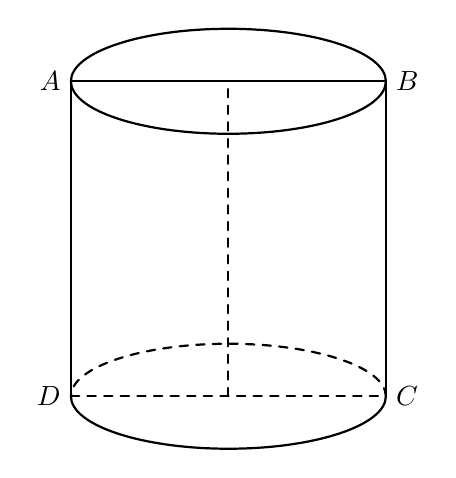
\begin{tikzpicture}[line join = round, line cap = round, scale = 1, thick]
				\pgfmathsetmacro\r{2};
				\draw (-\r, 0) node[left]{$D$} arc (180:360:{\r} and {\r/3});
				\draw[dashed] (\r,0) node[right]{$C$} arc (0:180:{\r} and {\r/3});
				\draw (-\r,4)  node[left]{$A$} arc (180:360:{\r} and {\r/3});
				\draw (\r,4) node[right]{$B$} arc (0:180:{\r} and {\r/3});
				\draw (-\r,0)--(-\r,4)--(\r,4)--(\r,0);
				\draw[dashed] (-\r,0)--(\r,0) (0,0)--(0,4);
			\end{tikzpicture}
		}
	}
\end{ex}

\begin{ex}%[2H2B1-2]
	Trong không gian cho hình chữ nhật $ABCD$ có $AB = a$ và $AD = 2a$. Gọi $H, K$ lần lượt là trung điểm của $AD$ và $BC$. Quay hình chữ nhật đó quanh trục $HK$, ta được một hình trụ. Diện tích toàn phần của hình trụ là
	\choice
	{$8\pi$}
	{$8a^2\pi$}
	{\True $4a^2\pi$}
	{$4\pi$}
	\loigiai{
		\immini{Khi quay hình chữ nhật $ABCD$ quanh trục $HK$ ta được hình trụ có bán kính đáy $R=HD=a$, chiều cao $h=HK=a$.\\
			Diện tích toàn phần của hình trụ là
			$$S_{tp} = 2\pi Rh + 2\pi R^2 = 4\pi a^2.$$
		}
		{
			\begin{tikzpicture}[line join = round, line cap = round, scale = 1]
				\path (-2,2) coordinate (A) node[above left]{$A$}
				(0,2) coordinate (H) node[above]{$H$}
				(2,2) coordinate (B) node[above right]{$D$}
				(2,0) coordinate (C) node[below right]{$C$}
				(0,0) coordinate (K) node[below]{$K$}
				(-2,0) coordinate (D)node[below left]{$B$};
				\draw (A)--(B)--(C)--(D)--(A) (H)--(K);
			\end{tikzpicture}
		}
	}
\end{ex}

\begin{ex}%[2H2B1-2][Lê Quý Đôn - Hải Phòng - 2018]
	Cho hình chữ nhật $ABCD$ có $AB = a$, $AD = 2a$. Gọi $M, N$ lần lượt là trung điểm của các cạnh $BC$ và $AD$. Khi quay hình chữ nhật trên (kể cả các điểm bên trong của nó) quanh đường thẳng $MN$ ta nhận được một khối tròn xoay $(T)$. Tính thể tích của $(T)$ theo $a$.
	\choice
	{$\dfrac{4\pi a^3}{3}$}
	{$\dfrac{\pi a^3}{3}$}
	{\True $\pi a^3$}
	{$4\pi a^3$}
	\loigiai{\immini{Khối tròn xoay nhận được là khối trụ có bán kính đáy $r=MC=a$, chiều cao $h=MN=a$.\\
			Thể tích khối tròn xoay $(T)$ là $$V=\pi r^2h=\pi a^2.a=\pi a^3.$$
		}{
			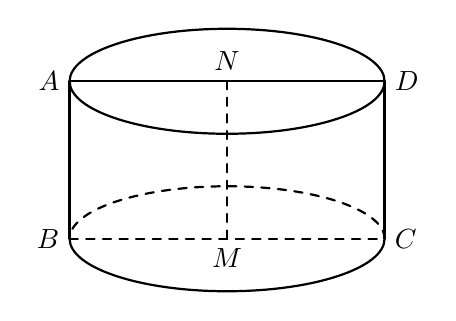
\begin{tikzpicture}[line join = round, line cap = round, scale = 1, thick]
				\pgfmathsetmacro\r{2};
				\draw (-\r, 0) node[left]{$B$} arc (180:360:{\r} and {\r/3});
				\draw[dashed] (\r,0) node[right]{$C$} arc (0:180:{\r} and {\r/3});
				\draw (-\r,2)  node[left]{$A$} arc (180:360:{\r} and {\r/3});
				\draw (\r,2) node[right]{$D$} arc (0:180:{\r} and {\r/3});
				\draw (-\r,0)--(-\r,2)--(\r,2)--(\r,0);
				\draw[dashed] (-\r,0)--(\r,0) (0,0) node[below]{$M$}--(0,2) node[above]{$N$};
			\end{tikzpicture}
		}
	}
\end{ex}

\begin{ex}%[2H2B1-2][Chuyên Vinh - 2018]
	Cho hình trụ có bán kính đáy bằng $R$, chiều cao bằng $h$.
	Biết rằng hình trụ đó có diện tích toàn phần gấp đôi diện tích xung quanh. Mệnh đề nào sau	đây đúng?
	\choice
	{\True $R=h$}
	{$R=2h$}
	{$h=2R$}
	{$h=\sqrt{2}R$}
	\loigiai{Ta có $S_{tp}=2S_{xq}\Leftrightarrow 2\pi R^2 + 2\pi Rh = 2.2\pi Rh \Leftrightarrow R = h.$}
\end{ex}

%%%--30-38
\begin{ex}%[2H2B1-2]
	Cho hình trụ có bán kính đáy bằng $R$ và chiều cao bằng $\dfrac{3R}{2}$. Mặt phẳng $(\alpha)$ song song với trục của hình trụ và cách trục một khoảng bằng $\dfrac{R}{2}$. Tính thiết diện của hình trụ cắt bởi mặt phẳng $(\alpha)$.
	\choice
	{$\dfrac{2R^2\sqrt{3}}{3}$}
	{\True $\dfrac{3R^2\sqrt{3}}{2}$}
	{$\dfrac{3R^2\sqrt{2}}{2}$}
	{$\dfrac{2R^2\sqrt{2}}{3}$}
	\loigiai{
		\begin{center}
			\begin{tikzpicture}[font=\footnotesize]
				\draw (0,0) ellipse (2cm and 0.6cm);
				\draw (-2,0) -- (-2,-4);
				\draw (2,0) -- (2,-4);
				\draw (-2,-4) arc (180:360:2cm and 0.6cm);
				\draw[dashed] (2,-4) arc (0:180:2cm and 0.6cm);
				\fill (0,0) circle (1.5pt);
				\fill (0,-4) circle (1.5pt);
				\node[draw,fill,circle,inner sep=1pt,label={-100:$A$}] (A) at (-70:2cm and 0.6cm) {};
				\node[draw,fill,circle,inner sep=1pt,label={90:$B$}] (B) at (45:2cm and 0.6cm) {};
				\node[draw,fill,circle,inner sep=1pt,label={-90:$D$}] at ($(0,-4)+(-70:2 and 0.6)$) {};
				\node[draw,fill,circle,inner sep=1pt,label={30:$C$}] at ($(0,-4)+(45:2 and 0.6)$) {};
				\draw (-70:2cm and 0.6cm) -- ($(0,-4)+(-70:2 and 0.6)$);
				\draw (-70:2cm and 0.6cm) -- (45:2cm and 0.6cm);
				\draw[dashed] ($(0,-4)+(-70:2 and 0.6)$) -- ($(0,-4)+(45:2 and 0.6)$) -- (45:2cm and 0.6cm);
				\node[above] at (0,0) {$O$};
				\node[below] at (0,-4) {$O'$};
				%				\fill (2,0) circle (1.5pt);
				\coordinate (H) at ($(A)!0.5!(B)$);
				\node[draw,fill,circle,inner sep=1pt,label={90:$H$}] at (H) {};
				\draw (A) -- (0,0) -- (H);
				\draw[dashed] (0,0) -- (0,-4);
			\end{tikzpicture}
		\end{center}
		Thiết diện của hình trụ cắt bởi mặt phẳng $(\alpha)$ là hình chữ nhật $ABCD$ với $BC\dfrac{3R}{2}$.\\
		Gọi $H$ là trung điểm $A B$, ta có $O H=\dfrac{R}{2} \Rightarrow A B=2 HA=2 \sqrt{R^2-OH^2}=R \sqrt{3}$.\\
		Vậy diện tích thiết diện là: $S=A B \cdot BC=R \sqrt{3} \cdot \dfrac{3 R}{2}=\dfrac{3 R^2 \sqrt{3}}{2}$.
	}
\end{ex}
\begin{ex}%[2H2B1-2]
	Cắt hình trụ $(T)$ bằng một mặt phẳng đi qua trục được thiết diện là một hình chữ nhật có diện tích bằng $20$ cm$^2$ và chu vi bằng $18$ cm. Biết chiều dài của hình chữ nhật lớn hơn đường kính mặt đáy của hình trụ $(T)$. Diện tích toàn phần của hình trụ là:
	\choice
	{$30 \pi$ cm$^2$}
	{\True $28 \pi$ cm$^2$}
	{$24 \pi$ cm$^2$}
	{$26 \pi$ cm$^2$}
	\loigiai{
		\begin{center}
			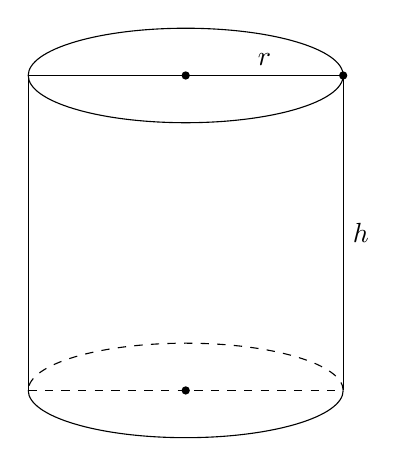
\begin{tikzpicture}
				\draw (0,0) ellipse (2cm and 0.6cm);
				\draw (-2,0) -- (-2,-4);
				\draw (2,0) -- (2,-4);
				\draw (-2,-4) arc (180:360:2cm and 0.6cm);
				\draw[dashed] (2,-4) arc (0:180:2cm and 0.6cm);
				\fill (0,0) circle (1.5pt);
				\fill (0,-4) circle (1.5pt);
				\node[above] at (1,0) {\normalsize$r$};
				\node[right] at (2,-2) {\normalsize$h$};
				\fill (2,0) circle (1.5pt);
				\draw[dashed] (-2,-4) -- (2,-4);
				\draw (-2,0) -- (2,0);
			\end{tikzpicture}
		\end{center}
		Gọi $ h$ và $ r$ là chiều cao và bán kính của hình trụ $ h>2 r$.\\
		Ta có $\heva{& 2rh=20 \\ & 2r+h=9}\Leftrightarrow \heva{& h=5 \\ & r=2}$.\\
		$S_{tp}=2\pi rh+2r^2\pi=20\pi +8\pi =28\pi$.
	}
\end{ex}
\begin{ex}%[2H1B1-2]
	Cắt hình trụ $(T)$ bởi một mặt phẳng qua trục của nó, ta được thiết diện là một hình vuông cạnh bằng $1$. Diện tích xung quanh của $(T)$ bằng.
	\choice
	{\True $\pi$}
	{$\dfrac{\pi}{2}$}
	{$2 \pi$}
	{$\dfrac{\pi}{4}$}
	\loigiai{
		\begin{center}
			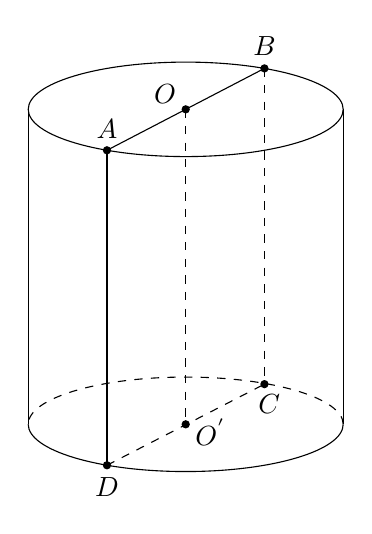
\begin{tikzpicture}
				\draw (0,0) ellipse (2cm and 0.6cm);
				\draw (-2,0) -- (-2,-4);
				\draw (2,0) -- (2,-4);
				\draw (-2,-4) arc (180:360:2cm and 0.6cm);
				\draw[dashed] (2,-4) arc (0:180:2cm and 0.6cm);
				\node[left] at (0,0.2) {\normalsize$O$};
				\fill (0,0) circle (1.5pt);
				\node[right] at (0,-4.1) {\normalsize$O^{'}$};
				\fill (0,-4) circle (1.5pt);
				\draw[dashed] (0,0) -- (0,-4);
				\fill (1,0.52) circle (1.5pt);
				\node at (-1,-0.25) {\normalsize$A$};
				\fill (-1,-0.52) circle (1.5pt);
				\node at (1,0.8) {\normalsize$B$};
				\draw (1,0.52) -- (-1,-0.52);
				\fill (1,-3.49) circle (1.5pt);
				\node[below right] at (0.8,-3.5) {\normalsize$C$};
				\fill (-1,-4.52) circle (1.5pt);
				\node at (-1,-4.8) {\normalsize$D$};
				\draw[dashed] (-1,-4.52) -- (1,-3.49);
				\draw[dashed] (1,0.52) -- (1,-3.49);
				\draw (-1,-0.52) -- (-1,-4.52);
			\end{tikzpicture}
		\end{center}
		Thiết diện qua trục là hình vuông $A B C D$ cạnh $ a$.\\
		Do đó hình trụ có đường cao $ h=1$ và bán kính đáy $ r=\dfrac{C D}{2}=\dfrac{1}{2}$.\\
		Diện tích xung quanh hình trụ: $S_{x q}=2 \pi r h=2 \pi \cdot 1 \cdot \dfrac{1}{2}=\pi$
	}
\end{ex}
\begin{ex}%[2H2B1-2]
	Cắt hình trụ $(T)$ bởi mặt phẳng qua trục của nó, ta được thiết diện là một hình vuông cạnh bằng 3. Diện tích xung quanh của $(T)$ bằng
	\choice
	{$\dfrac{9 \pi}{4}$}
	{$18 \pi$}
	{\True $9 \pi$}
	{$\dfrac{9 \pi}{2}$}
	\loigiai{
		Vì thiết diện qua trục của hình trụ $(T)$ là một hình vuông cạnh bằng 3 nên hình trụ $(T)$ có đường sinh $l=3$, bán kính $ r=\dfrac{l}{2}=\dfrac{3}{2}$.\\
		Diện tích xung quanh của hình trụ $(T)$ là $S_{x q}=2 \pi r l=2 \pi \cdot \dfrac{3}{2} \cdot 3=9 \pi$.
	}
\end{ex}
\begin{ex}%[2H2B1-2]
	Cắt hình trụ $(T)$ bởi một mặt phẳng qua trục của nó ta được thiết diện là một hình vuông cạnh bằng $7$. Diện tích xung quanh của $(T)$ bằng
	\choice
	{$\dfrac{49 \pi}{4}$}
	{$\dfrac{49 \pi}{2}$}
	{\True $49 \pi$}
	{$98 \pi$}
	\loigiai{
		Bán kính đáy của hình trụ là $ r=\dfrac{7}{2}$.
		Đường cao của hình trụ là $ h=7$.\\
		Diện tích xung quanh của hình trụ là $S=2 \pi r h=2 \pi \cdot \dfrac{7}{2} \cdot 7=49 \pi$.
	}
\end{ex}
\begin{ex}%[2H2B1-2]
	Cắt hình trụ $(T)$ bởi một mặt phẳng qua trục của nó, ta được thiết diện là một hình vuông cạnh bằng $5$. Diện tích xung quanh của $(T)$ bằng
	\choice
	{$\dfrac{25 \pi}{2}$}
	{\True $25 \pi$}
	{$50 \pi$}
	{$\dfrac{25 \pi}{4}$}
	\loigiai{
		\begin{center}
			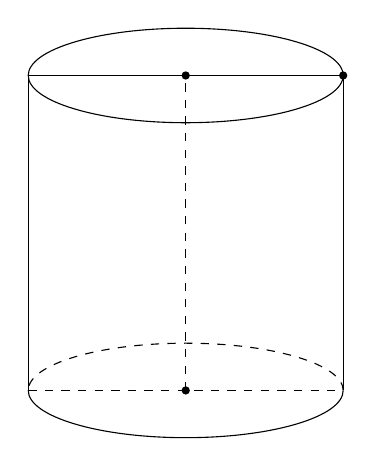
\begin{tikzpicture}
				\draw (0,0) ellipse (2cm and 0.6cm);
				\draw (-2,0) -- (-2,-4);
				\draw (2,0) -- (2,-4);
				\draw (-2,-4) arc (180:360:2cm and 0.6cm);
				\draw[dashed] (2,-4) arc (0:180:2cm and 0.6cm);
				\fill (0,0) circle (1.5pt);
				\fill (0,-4) circle (1.5pt);
				\fill (2,0) circle (1.5pt);
				\draw[dashed] (-2,-4) -- (2,-4);
				\draw (-2,0) -- (2,0);
				\draw[dashed] (0,-4) -- (0,0);
			\end{tikzpicture}
		\end{center}
		Bán kính của hình trụ $(T)$ bằng $\dfrac{5}{2}$, độ dài đường $\sinh l=5$.\\
		Diện tích xung quanh của $(T)$: $S_{x q}=2 \pi r \cdot l=2 \pi \cdot \dfrac{5}{2} \cdot 5=25 \pi$.
	}
\end{ex}
\begin{ex}%[2H2Y1-2]
	Một hình trụ có bán kính đáy $r=4$ cm và có độ dài đường sinh $l=3$ cm. Diện tích xung quanh của hình trụ đó bằng
	\choice
	{$12 \pi $ cm$^2$}
	{$48 \pi $ cm$^2$}
	{\True $24 \pi $ cm$^2$}
	{$36 \pi $ cm$^2$}
	\loigiai{
		Diện tích xung quanh của hình trụ là $S_{x q}=2 \pi r l=2 \pi 4\cdot 3=24$ cm$^2$.
	}
\end{ex}
\begin{ex}%[2H2Y1-2]
	Cho hình trụ có bán kính đáy $r$ và độ dài đường sinh $l$. Diện tích xung quanh $S$ của hình trụ đã cho được tính theo công thức nào dưới đây?
	\choice
	{$S_{x q}=4 \pi r l$}
	{\True $S_{x q}=2 \pi r l$}
	{$S_{x q}=3 \pi r l$}
	{$S_{x q}=\pi r l$}
	\loigiai{
		Công thức tính diện tích xung quanh của hình trụ là $S_{x q}=2 \pi r l$.
	}
\end{ex}
\begin{ex}%[2H2Y1-2]
	Cho hình trụ có chiều cao $ h=1$ và bán kính $ r=2$. Diện tích xung quanh của hình trụ đã cho bằng
	\choice
	{\True $4 \pi$}
	{$2 \pi$}
	{$3 \pi$}
	{$6 \pi$}
	\loigiai{
		Ta có $S_{x q}=2 \pi r h=4 \pi$.
	}
\end{ex}

%\Closesolutionfile{ans}
%\begin{indapan}{10}
%	{ans/CD-22-MD5.6}
%\end{indapan}

\begin{dang}{Tính thể tích khối trụ, khối nón.}
\end{dang}
\Opensolutionfile{ans}[ans/CD-22-MD5.6-2]
\begin{ex}%[2H2Y1-1]%[Mã 101-2021-Lần 1]
	Cho khối trụ có bán kính đáy $r=6$ và chiều cao $h=3$. Thể tích của khối trụ đã cho bằng
	\choice 
	{\True$108 \pi$}
	{$36 \pi$}
	{ $18 \pi$}
	{ $54 \pi$}
	\loigiai
	{Thể tích của khối trụ đã cho là $V=\pi r^2 h=\pi.6^2.3=108 \pi.$}
\end{ex}
\begin{ex} %[2H2Y1-1]%[Mã 103 - 2021 - Lần 1]%Câu 2
	Cho khối trụ có bán kính $r=2$ và chiều cao $h=3$.Thể tích khối trụ đã cho bằng
	\choice
	{\True$12 \pi$}
	{ $18 \pi$}
	{ $6 \pi$}
	{ $4 \pi$}
	\loigiai
	{Thể tích khối trụ: $V=\pi r^2 h=\pi.2^2.3=12 \pi.$}
\end{ex}

\begin{ex} %[2H2Y1-1]%[Mã $101-2020$ Lần 2]%Câu 3
	Cho khối trụ có bán kính đáy $r=4$ và chiều cao $h=3$. Thể tích của khối trụ đã cho bằng
	\choice 
	{ \True$48 \pi$}
	{ $4 \pi$}
	{ $16 \pi$}
	{ $24 \pi$}
	\loigiai
	{Thể tích khối trụ là $V=\pi r^2 h=\pi. 4^2.3=48 \pi.$}
\end{ex}

\begin{ex} %[2H2Y1-1]%[Mã $102-2020$ Lần 2]%Câu 4
	Cho khối trụ có bán kính đáy bằng $r=5$ và chiều cao $h=3$. Thể tích của khối trụ đã cho bằng
	\choice 
	{ $5 \pi$}
	{ $30 \pi$}
	{ $25 \pi$}
	{ \True$75 \pi$}
	\loigiai
	{Thể tích khối trụ là $V=\pi r^2.h=75 \pi.$}
\end{ex}

\begin{ex} %[2H2Y1-1]%[Mã 103 - 2020 Lần 2]%Câu 5
	Cho khối trụ có bán kính $r=3$ và chiều cao $h=4$. Thể tích khối trụ đã cho bằng
	\choice 
	{ $4 \pi$}
	{ $12 \pi$}
	{ \True$36 \pi$}
	{ $24 \pi$}
	\loigiai
	{Ta có: $V=\pi r^2 h=\pi .3^2 .4=36 \pi.$}
\end{ex}

\begin{ex} %[2H2Y1-1]%[Mã 104-2020 Lần 2]%Câu 6
	Cho khối trụ có bán kính đáy $r=3$ và chiều cao $h=5$. Thể tích của khối trụ đã cho bằng
	\choice 
	{ \True$45 \pi$}
	{ $5 \pi$}
	{ $15 \pi$}
	{ $30 \pi$}
	\loigiai
	{Thể tích của khối trụ đã cho là: $V=Bh=\pi r^2 h=\pi. 3^2.5=45 \pi.$}
\end{ex}

\begin{ex} %[2H2Y1-1]%[Mã 103 2018]%Câu 7 
	Thể tích của khối trụ tròn xoay có bán kính đáy $r$ và chiều cao $h$ bằng
	\choice 
	{ $\dfrac{4}{3} \pi r^2 h$}
	{ \True$\pi r^2 h$}
	{ $\dfrac{1}{3} \pi r^2 h$}
	{ $2 \pi r h$}
	\loigiai
	{$\bar{V}_{t r u}=\pi r^2 h $.}
\end{ex}

\begin{ex} %[2H2Y1-1]%[Mã 123 2017]%Câu 8 
	Tính thể tích $V$ của khối trụ có bán kính $r=4$ và chiều cao $h=4 \sqrt{2}$.
	\choice 
	{ $V=32 \pi$}
	{ \True $V=64 \sqrt{2} \pi$}
	{ $V=128 \pi$}
	{ $V=32 \sqrt{2} \pi$}
	\loigiai
	{$V=\pi r^2 h=16.4 \sqrt{2} \pi=64 \sqrt{2} \pi$.}
\end{ex}

\begin{ex} %[2H2Y1-1]%[Chuyên Lê Hồng Phong Nam Định 2019]%Câu 9
	Thể tích khối trụ có bán kính đáy $r=a$ và chiều cao $h=a \sqrt{2}$ bằng
	\choice 
	{ $4 \pi a^3 \sqrt{2}$}
	{ \True $\pi a^3 \sqrt{2}$}
	{ $2 \pi a^3$}
	{ $\dfrac{\pi a^3 \sqrt{2}}{3}$}
	\loigiai
	{\immini{	Thể tích khối trụ là: $V=\pi r^2 h=\pi .a^2 .a \sqrt{2}=\pi a^3 \sqrt{2}$.}
		{\begin{tikzpicture}[scale=.8,line join=round, line cap=round,font=\footnotesize]
				\def \x{1.8} %bán kính trục lớn elip
				\def \y{0.8} %bán kính trục bé elip
				\def \h{3.5} %chiều cao hình trụ
				\coordinate (A) at (0,0);
				\coordinate (B) at (2*\x,0);
				\coordinate (O) at ($(A)!0.5!(B)$);
				\coordinate (O') at ($(O)+(0,\h)$);
				\coordinate (A') at ($(A)+(0,\h)$);
				\coordinate (B') at ($(B)+(0,\h)$);
				\draw[dashed] (B) arc(0:180:\x cm and \y cm);
				\draw (B) arc(0:-180:\x cm and \y cm);
				\draw (O') ellipse (\x cm and \y cm);
				\tkzDrawSegments(A,A' B,B')
				\tkzDrawSegments[dashed](O,O')
				\tkzDrawSegments[dashed](O,B)
				\tkzDrawSegments(O',B')
				\tkzLabelSegment(O,B){$r=a$}
				\tkzLabelSegment[right](B',B){$h=a\sqrt{2}$}
				\tkzDrawPoints[fill=black,size=3](A,B,O,O',A',B')
				\tkzLabelPoints[left](A,A')
				\tkzLabelPoints[right](B,B')
				\tkzLabelPoints[above](O')
				\tkzLabelPoints[below](O)
		\end{tikzpicture} }
		
	}
\end{ex}	
\begin{ex} %[2H2Y1-1]%[Chuyên Lê Quý Đôn Điện Biên 2019] 
	Thiết diện qua trục của một hình trụ là một hình vuông có cạnh bằng $2 a$. Tính theo $a$ thể tích khối trụ đó
	\choice 
	{ $\pi a^3$}
	{ \True$2 \pi a^3$}
	{ $4 \pi a^3$}
	{ $\dfrac{2}{3} \pi a^3$}
	\loigiai
	{Gọi chiều cao và bán kính đáy của hình trụ lần lượt là $h, r$.\\
		Thiết diện qua trục của hình trụ là một hình vuông có cạnh bằng $2 a$ nên $h=2 a, r=a$.\\
		Thể tích của khối trụ đó là $V=\pi r^2 h=\pi a^2 .2 a=2 \pi a^3$.}
\end{ex}

\begin{ex} %[2H2Y1-1] (THPT lê Quý Đôn Đà Nẵng 2019)
	Cho hình chữ nhật $ABCD$ có $AB=2, BC=2a$. Tính thể tích khối tròn xoay khi quay hình phẳng $ABCD$ quanh trục $AD$.
	\choice 
	{\True $4 \pi a^3$}
	{ $2 \pi a^3$}
	{ $8 \pi a^3$}
	{ $\pi a^3$}
	\loigiai
	{Khối tròn xoay tạo thành là khối trụ có bán kính đáy là $A B=2 a$ và đường cao $A D=B C=a$ có thể tích bằng $V=\pi A B^2 A D=4 \pi a^3$.}
\end{ex}

%%---12-22
\begin{ex}%[2H2B1-2]%Câu 1
	Cho hình chữ nhật $ABCD$ có $AB=2BC=2a$. Tính thể tích khối tròn xoay khi quay hình phẳng $ABCD$ quanh trục $AD.$
	\choice
	{\True $4\pi a^3$}
	{$2\pi a^3$}
	{$8\pi a^3$}
	{$\pi a^3$}
	\loigiai{
		Khối tròn xoay tạo thành là khối trụ có bán kính đáy là $AB$ có $a=2$ và đường cao $AD=BC=a$ có thể tích bằng $V=\pi AB^2.AD=4\pi a^3$.}
\end{ex}

\begin{ex}%[2H2B1-2]%Câu 2
	Cho hình trụ có diện tích toàn phần là $4\pi$ và có thiết diện cắt bởi mặt phẳng qua trục là hình vuông. Tính thể tích khối trụ?
	\choice
	{$\frac{\pi \sqrt{6}}{12}$}
	{$\frac{\pi \sqrt{6}}{9}$}
	{$\frac{4\pi}{9}$}
	{\True $\frac{4\pi \sqrt{6}}{12}$}
	\loigiai{Hình trụ có thiết diện cắt bởi mặt phẳng qua trục là hình vuông suy ra $l=h=2r$ \\ Hình trụ có diện tích toàn phần là $4\pi$ suy ra \\ $S_{tp}=2\pi rl+2\pi r^2=2\pi .2r^2+2\pi r^2=4\pi r^2=4\pi$ \\ Nên $r=\frac{\sqrt{6}}{3}, l=h=\frac{2\sqrt{6}}{3}$ \\ Thể tích khối trụ $V=\pi r^2h=\frac{4\pi \sqrt{6}}{12}$.}
\end{ex}

\begin{ex}%[2H2B1-2]%Câu 3
	Cho hình chữ nhật $ABCD$ có $AB=a, AD=2a$. Tính thể tích khối trụ tạo thành khi quay hình chữ nhật $ABCD$ quanh cạnh $AB.$
	\choice
	{\True $4\pi a^3$}
	{$\pi a^3$}
	{$3 a^3$}
	{$a^3$}
	\loigiai{
		Áp dụng công thức tính thể tích khối trụ tròn xoay ta có \\ $V=\pi r^2h=\pi (2a)^2.a=\pi a^3$.}
\end{ex}

\begin{ex}%[2H2B1-2]%Câu 4
	Trong không gian, cho hình chữ nhật $ABCD$ có $AB=1, AD=2$. Gọi $M, N$ lần lượt là trung điểm $AB, CD$. Quay hình chữ nhật đó xung quanh trục $MN$ ,ta được một hình trụ. Tính thể tích $V$ của khối trụ tạo bởi hình trụ đó
	\choice
	{\True $\frac{\pi}{2}$}
	{$ \pi$}
	{$2 \pi$}
	{$4\pi$}
	\loigiai{
		\begin{center}
			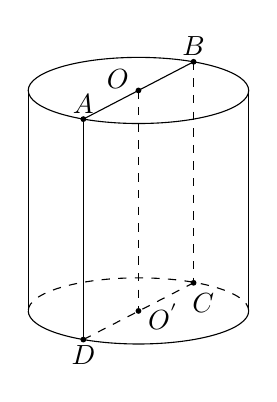
\begin{tikzpicture}[scale=.7]
				\draw (0,0) ellipse (2cm and 0.6cm);
				\draw (-2,0) -- (-2,-4);
				\draw (2,0) -- (2,-4);
				\draw (-2,-4) arc (180:360:2cm and 0.6cm);
				\draw[dashed] (2,-4) arc (0:180:2cm and 0.6cm);
				\node[left] at (0,0.2) {\normalsize$O$};
				\fill (0,0) circle (1.5pt);
				\node[right] at (0,-4.1) {\normalsize$O^{'}$};
				\fill (0,-4) circle (1.5pt);
				\draw[dashed] (0,0) -- (0,-4);
				\fill (1,0.52) circle (1.5pt);
				\node at (-1,-0.25) {\normalsize$A$};
				\fill (-1,-0.52) circle (1.5pt);
				\node at (1,0.8) {\normalsize$B$};
				\draw (1,0.52) -- (-1,-0.52);
				\fill (1,-3.49) circle (1.5pt);
				\node[below right] at (0.8,-3.5) {\normalsize$C$};
				\fill (-1,-4.52) circle (1.5pt);
				\node at (-1,-4.8) {\normalsize$D$};
				\draw[dashed] (-1,-4.52) -- (1,-3.49);
				\draw[dashed] (1,0.52) -- (1,-3.49);
				\draw (-1,-0.52) -- (-1,-4.52);
			\end{tikzpicture}
		\end{center}
		Quay hình chữ nhật xung quanh trục $MN$ ta được hình trụ có bán kính đáy $r=AM=\frac{1}{2}$, chiều cao $h=AD=2$. Thể tích khối trụ tương ứng bằng $V=\pi r^2h=\pi \left(\frac{1}{2}\right)^2.2=\frac{\pi}{2}$.
	}
\end{ex}

\begin{ex}%[2H2B1-2]%Câu 5
	Cho khối trụ có chu vi đáy bằng $4\pi a$ và độ dài đường cao bằng $a$. Thể tích của khối trụ đã cho bằng
	\choice
	{$\pi a^3$}
	{$\frac{4}{3}\pi a^3$}
	{\True$4\pi a^3$}
	{$16\pi a^3$}
	\loigiai{Gọi chu vi đáy là $P=2\pi R\Leftrightarrow 4\pi a=2 \pi R\Leftrightarrow R=2a$. \\ Khi đó, thể tích của khối trụ $V=\pi R^2h=\pi (2\pi)^2.2=4\pi a^3$.}
\end{ex}

\begin{ex}%[2H2B1-2]%Câu 6
	Cho một khối trụ có diện tích xung quanh của khối trụ bằng $80\pi$. Tính thể tích của khối trụ biết khoảng các hai đáy bằng 10.
	\choice
	{$\pi a^2$}
	{$\frac{4}{3}\pi a^3$}
	{\True $4\pi a^2$}
	{$16\pi a^3$}
	\loigiai{
		\begin{center}
			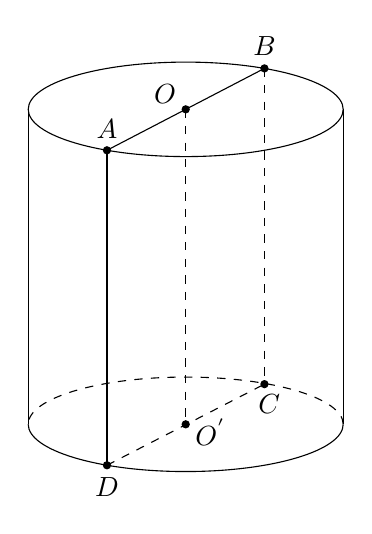
\begin{tikzpicture}
				\draw (0,0) ellipse (2cm and 0.6cm);
				\draw (-2,0) -- (-2,-4);
				\draw (2,0) -- (2,-4);
				\draw (-2,-4) arc (180:360:2cm and 0.6cm);
				\draw[dashed] (2,-4) arc (0:180:2cm and 0.6cm);
				\node[left] at (0,0.2) {\normalsize$O$};
				\fill (0,0) circle (1.5pt);
				\node[right] at (0,-4.1) {\normalsize$O^{'}$};
				\fill (0,-4) circle (1.5pt);
				\draw[dashed] (0,0) -- (0,-4);
				\fill (1,0.52) circle (1.5pt);
				\node at (-1,-0.25) {\normalsize$A$};
				\fill (-1,-0.52) circle (1.5pt);
				\node at (1,0.8) {\normalsize$B$};
				\draw (1,0.52) -- (-1,-0.52);
				\fill (1,-3.49) circle (1.5pt);
				\node[below right] at (0.8,-3.5) {\normalsize$C$};
				\fill (-1,-4.52) circle (1.5pt);
				\node at (-1,-4.8) {\normalsize$D$};
				\draw[dashed] (-1,-4.52) -- (1,-3.49);
				\draw[dashed] (1,0.52) -- (1,-3.49);
				\draw (-1,-0.52) -- (-1,-4.52);
			\end{tikzpicture}
		\end{center}
		Ta có khoảng cách giữa hai đáy bằng 10 nên $h=l=10.$\\ $S_{xq}=80\pi \Leftrightarrow 2\pi rl=20\pi \Leftrightarrow r=4$. \\ Vậy thể tích của khối trụ bằng $V=\pi 4^2.10=160\pi$.
	}
\end{ex}

\begin{ex}%[2H2B1-2]%Câu 7
	Cho khối trụ có bán kính hình tròn đáy bằng $r$ và chiều cao bằng $h$ . Hỏi nếu tăng chiều cao lên 2 lần và tăng bán kính đáy lên 3 lần thì thể tích của khối trụ mới sẽ tăng lên bao nhiêu lần?
	\choice
	{\True 18 lần}
	{6 lần}
	{36 lần}
	{12 lần}
	\loigiai{$V_1=2h\pi (3r)^2=18\left(h\pi r^2\right)=18V$.}
\end{ex}

\begin{ex}%[2H2B1-2]%Câu 8
	Mặt phẳng đi qua trục hình trụ, cắt hình trụ theo thiết diện là hình vuông cạnh $a$ . Thể tích khối trụ đó bằng
	\choice
	{$\pi a^3$}
	{\True $\frac{\pi a^3}{2}$}
	{$\frac{\pi a^3}{2}$}
	{$16\pi a^3$}
	\loigiai{
		\begin{center}
			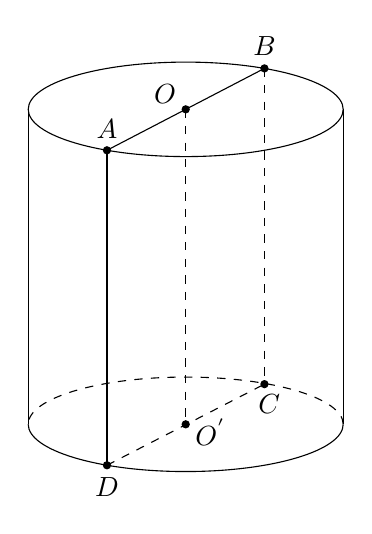
\begin{tikzpicture}
				\draw (0,0) ellipse (2cm and 0.6cm);
				\draw (-2,0) -- (-2,-4);
				\draw (2,0) -- (2,-4);
				\draw (-2,-4) arc (180:360:2cm and 0.6cm);
				\draw[dashed] (2,-4) arc (0:180:2cm and 0.6cm);
				\node[left] at (0,0.2) {\normalsize$O$};
				\fill (0,0) circle (1.5pt);
				\node[right] at (0,-4.1) {\normalsize$O^{'}$};
				\fill (0,-4) circle (1.5pt);
				\draw[dashed] (0,0) -- (0,-4);
				\fill (1,0.52) circle (1.5pt);
				\node at (-1,-0.25) {\normalsize$A$};
				\fill (-1,-0.52) circle (1.5pt);
				\node at (1,0.8) {\normalsize$B$};
				\draw (1,0.52) -- (-1,-0.52);
				\fill (1,-3.49) circle (1.5pt);
				\node[below right] at (0.8,-3.5) {\normalsize$C$};
				\fill (-1,-4.52) circle (1.5pt);
				\node at (-1,-4.8) {\normalsize$D$};
				\draw[dashed] (-1,-4.52) -- (1,-3.49);
				\draw[dashed] (1,0.52) -- (1,-3.49);
				\draw (-1,-0.52) -- (-1,-4.52);
			\end{tikzpicture}
		\end{center}
		Ta có bán kính đáy $r=\frac{a}{2}$ và chiều cao $h=1$ nên thể tích khối trụ là \\ $V=2\pi r^2h=2\pi \frac{a^2}{4}a=\frac{\pi a^3}{2}$
	}
\end{ex}

\begin{ex}%[2H2B1-2]%Câu 9
	Thiết diện qua trục của một hình trụ là hình vuông có cạnh là $2a$ .Thể tích khối trụ được tạo nên bởi hình trụ này là:
	\choice
	{\True $2\pi a^3$}
	{$\frac{2\pi a^3}{3}$}
	{$8\pi a^3$}
	{$\frac{8\pi a^3}{3}$}
	\loigiai{Ta có $R=a, h=2a$, nên thể tích khối trụ được tạo nên bởi hình trụ này là \\ $V=\pi R^2h=\pi a^2.2a=2\pi a^3$.}
\end{ex}

\begin{ex}%[2H2B1-2]%Câu 10
	Cho một khối trụ $(S)$ có bán kính đáy là $a$. Biết thiết diện của hình trụ qua trục là hình vuông có chu vi là 8. Thể tích của khối trụ sẽ bằng
	\choice
	{$8\pi$}
	{$4\pi$}
	{\True $2\pi$}
	{$16\pi$}
	\loigiai{Ta có chiều cao của khối trụ $h=2r=2a.$\\Theo giả thiết ta có $4.2a=8\Leftrightarrow a=1.$\\Thể tích khối trụ $V=\pi r^2h=\pi a^2.2a=2\pi.$}
\end{ex}

\begin{ex}%[2H2K1-2]%Câu 11
	Cắt một khối trụ bởi một mặt phẳng qua trục ta được thiết diện là hình chữ nhật $ABCD$ có $AB$ và $CD$ thuộc hai đáy của khối trụ. Biết $AB=4a, AC=5a$. Tính thể tích của khối trụ:
	\choice
	{\True $12\pi a^3$}
	{$16\pi a^3$}
	{$4\pi a^3$}
	{$8\pi a^3$}
	\loigiai{
		\begin{center}
			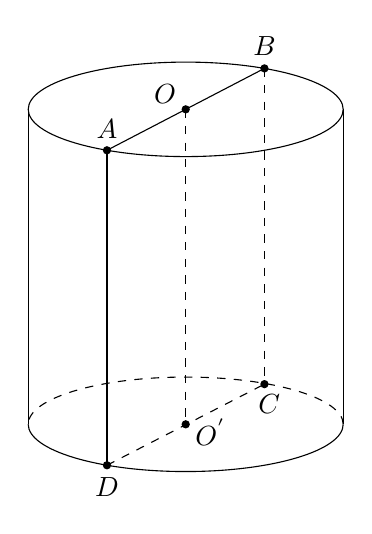
\begin{tikzpicture}
				\draw (0,0) ellipse (2cm and 0.6cm);
				\draw (-2,0) -- (-2,-4);
				\draw (2,0) -- (2,-4);
				\draw (-2,-4) arc (180:360:2cm and 0.6cm);
				\draw[dashed] (2,-4) arc (0:180:2cm and 0.6cm);
				\node[left] at (0,0.2) {\normalsize$O$};
				\fill (0,0) circle (1.5pt);
				\node[right] at (0,-4.1) {\normalsize$O^{'}$};
				\fill (0,-4) circle (1.5pt);
				\draw[dashed] (0,0) -- (0,-4);
				\fill (1,0.52) circle (1.5pt);
				\node at (-1,-0.25) {\normalsize$A$};
				\fill (-1,-0.52) circle (1.5pt);
				\node at (1,0.8) {\normalsize$B$};
				\draw (1,0.52) -- (-1,-0.52);
				\fill (1,-3.49) circle (1.5pt);
				\node[below right] at (0.8,-3.5) {\normalsize$C$};
				\fill (-1,-4.52) circle (1.5pt);
				\node at (-1,-4.8) {\normalsize$D$};
				\draw[dashed] (-1,-4.52) -- (1,-3.49);
				\draw[dashed] (1,0.52) -- (1,-3.49);
				\draw (-1,-0.52) -- (-1,-4.52);
			\end{tikzpicture}
		\end{center}
		Ta có bán kính hình khối trụ $R=\frac{AB}{2}=2a.$\\Xét $\Delta ADC$ vuông tại $D$: $AD=\sqrt{AC^2-DC^2}=\sqrt{(5a)^2-(4a)^2}=3a.$ \\ Thể tích khối trụ là $V=\pi R^2h=\pi (2a)^2.3a=12\pi a^3$.
	}
\end{ex}
\Closesolutionfile{ans}
\indapan{10}{ans/CD22/Muc_5_6}